

\begin{comment}
 In the second test, we prove the functionality of the algorithm in three dimensions. 

The algorithm compares the images and calculates the departure factor 
based on area of ROI. Fig. \ref{fig:target} demonstrates the 
tracking of $40$ images from initial position to the final position of the target, 
highlighted with red boxes;
the vector in blue describes the movement of the target. 

\begin{figure}[H]
\centering
  \subfloat[]{\label{fig:targeinit} \includegraphics[width=.48\columnwidth]{images/figurea.eps}}
  \subfloat[]{\label{fig:targeend} \includegraphics[width=.48\columnwidth]{images/figureb.eps}}
  \caption{The target in (a) is the initial position and its area is smaller than the target in (b), 
  which represents the final position. The factor is dividing both areas.}
  \label{fig:target}
\end{figure}

In Fig. \ref{fig:target}, we can observe an increase in ROI, and 
its influence to the departure factor is shown in Fig. \ref{fig:res_grapha_b}.

\begin{figure}[H]
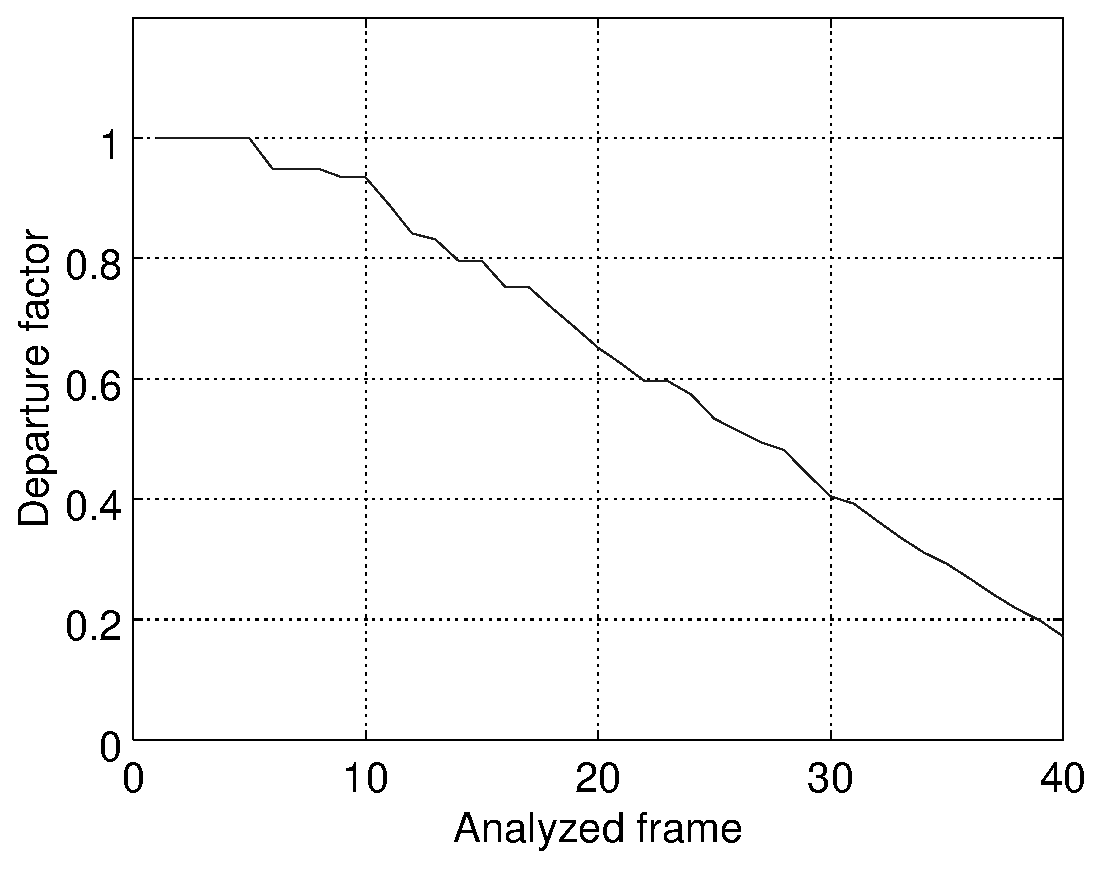
\includegraphics[width=\columnwidth]{images/grapha_b.eps}
\caption{Departure factor for each frame in the test 2.}
\label{fig:res_grapha_b}
\end{figure}

The Fig. \ref{fig:res_grapha_b} shows the departure factor in each frame
of test 2 (see the line with circles), additionally It is showed a polynomial
fitting of departure factor using a polynomial of order 4 (see the line with dots),
finally It is showed the real route of target normalized to $1.0$ for the maximum distance
(see the line with squares), as can be seen the target is approaching with a constant speed. 
If we interpret this value as the position in each sample time, 
then the departure factor describes the relative target position.
In the first image the analyzed target is at a distance $d_0$ 
and in the last image the target is at a distance of $17.18\%$ of $d_0$.
The departure distance decreases in discrete steps because the departure
factor is selected in discrete steps, if the target is
between two consecutive analysis layers (scales), the algorithm
approximates the target to the nearest layer.



The Table \ref{tab:tab1} represents the bank of images used for test 2, totally 40 images generated by POV-Ray.
The number of analyzed frames are in the first column of table, in the second column are the real distances 
between camera and target.
The percentage proportion of real distances are in third column. For example, 
the target in first frame is to $23.5$ meters from camera and it is considered the $100$\% of distance,
by other side, in the frame $40$ the target is to $4$ meters 
from camera and is $17,02$\% in relation of first frame. Next column, fourth column, 
we have the results of algorithm (departure factor), in the percentage form. 
%Note in first frame, target is $100$\% of distance and the last frame is at $17,18$\% of distance in relation of first frame.
Finally, the last column represents the error between percentage real distance and the departure factor. 
As can be seen, the error is diminishing when target is close (around 5 meters), it means that the algorithm has more precision 
when image of target is bigger because there are more information in ROI. It is a consequence of PCC, 
because in small ROI each pixel charge much information in comparative method. On other hand, if ROI is bigger,
the information is diluted around pixels; thus, the algorithm has more data to compare.
Another reason is that in the last frames $1$ pixel of target
represents a less distance in meters that $1$ pixel in the target of the first frames; consequently, the error 
of a quantity $x$ of pixels represents a less quantity of error meters in the analysis of last frames.

\begin{table}[H]
\setlength{\tabcolsep}{1 pt} 
\caption{Table of comparative results}
\begin{tabular}{lllll}
Frames & Real Dist. (m) & Real Dist. (\%) & Dep. factor (\%) & Relative error (\%)\\
1 & 23.5 & 100.0 & 100.0 & 0.0 \\
10 & 19.0 & 80.85 & 93.46 & 15.60 \\
20 & 14.0 & 59.57 & 65.16 & 9.37 \\
30 & 9.0 & 38.30 & 40.46 & 5.65 \\
40 & 4.0 & 17.02 & 17.18 & 0.93
\end{tabular}
\label{tab:tab1}
\end{table}

The Fig. \ref{fig:res_grapha_bv} shows the velocities of the data showed in the 
Fig. \ref{fig:res_grapha_b}  calculated to $d_0=1$ and $\Delta t=1$. 
Thus, it is showed the velocity of departure factor (see the line with circles), 
additionally It is showed the velocity of the polynomial
fitting of departure factor (see the line with dots) and
finally It is showed the velocity of the normalized real route
(see the line with squares), being it a constant.
The velocities were calculated using the discrete-time derivate.
The values of the velocities are negatives, which indicates that the
target is approaching towards the observer. As can be seen,
the velocity of the departure factor don't have a monotone behavior 
because that the curve of the departure factor has a many discrete changes; thus,
It is important to use the polynomial fitting curve
to calculate the velocity, because this curve represents
very close the behavior of the velocity of the normalized real route.

\begin{figure}[!hbt]
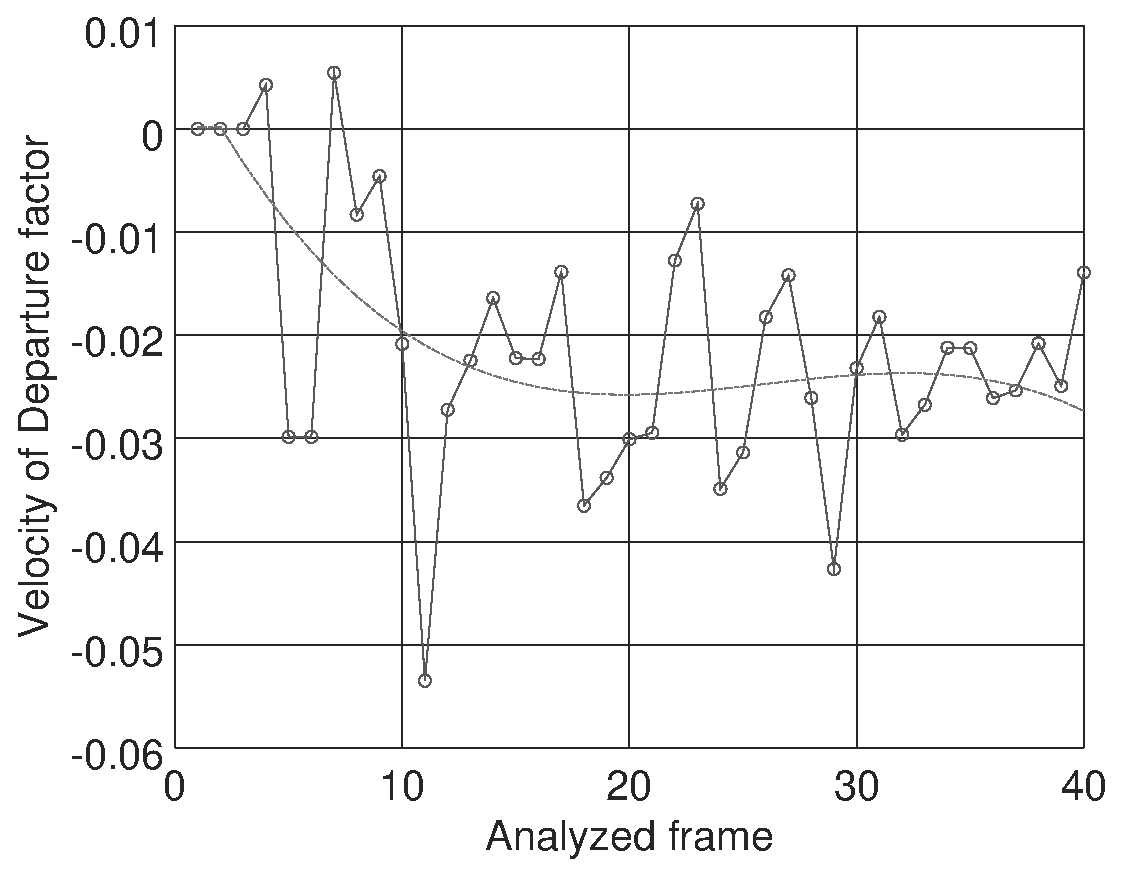
\includegraphics[width=\columnwidth]{images/graphvelocity.eps}
\caption{Velocity of departure factor for each frame in test 2.}
\label{fig:res_grapha_bv}
\end{figure}

\end{comment}


%%%%%%%%%%%%%%%%%%%%%%%%%%%%%%%%%%portugues%%%%%%%%%%%%%%%%%%%%%%%%%%%%%%%%%%%%%%%%%%%%%%%%
A funcionalidade do algoritmo é verificado no segundo teste.

O algoritmo compara as imagens e calcula o fator de aproximação, 
baseando-se na área do $ROI$. Fig. \ref{fig:target} representa o 
acompanhamento do objeto por $40$ imagens. Os retângulos vermelhos
são as posições inicial e final, ligados por um vetor em azul.

\begin{figure}[H]
\centering
  \subfloat[]{\label{fig:targeinit} \includegraphics[width=.48\columnwidth]{images/figurea.eps}}
  \subfloat[]{\label{fig:targeend} \includegraphics[width=.48\columnwidth]{images/figureb.eps}}
  \caption{O Objeto em (a) está na posição incial com área menor que (b), 
  posição final. O fator representa a proporção entre as duas áreas.}
  \label{fig:target}
\end{figure}

Na fig. \ref{fig:target}, observa-se um crescimento no $ROI$ e, por
consequência, uma modificação do fator de aproximação na fig \ref{fig:res_grapha_b}.

\begin{figure}[H]
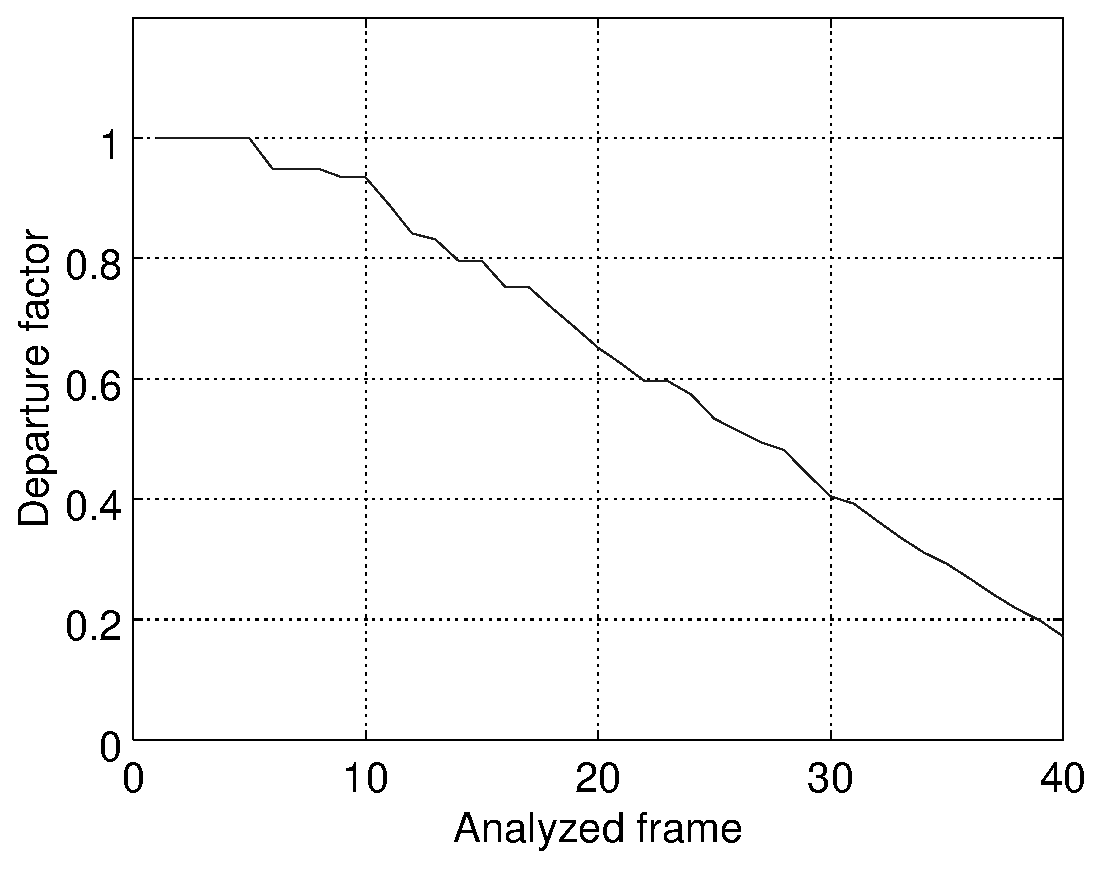
\includegraphics[width=\columnwidth]{images/grapha_b.eps}
\caption{O fator de aproximação para cada imagem no teste 2.}
\label{fig:res_grapha_b}
\end{figure}





A fig. \ref{fig:res_grapha_b} mostra o fator de aproximação em cada frame 
do teste 2 (veja a linha com círculos),
além disso, é mostrado um ajuste polinomial do fator de aproximação usando 
um polinômio de ordem 4 (veja a linha com pontos),
finalmente, mostra-se a rota real do alvo normalizada para $1,0$ na 
distância máxima (veja a linha com quadrados),
como pode ser visto, o alvo está se aproximando com uma velocidade constante.
Se for adotado esse valor normalizado como a posição do objeto para cada imagem, então o fator de aproximação
descreve a posição relativa do objeto.

Assim, na primeira imagem o objeto analisado está a uma distância $d_0$
e na última a uma distância $17.18\%$ de $d_0$.
A aproximação do objeto à câmera é discretizado, portanto se o objeto
estiver entre duas camadas de análises, o algoritmo aproxima o para
a camada mais próxima da câmera.

A tabela \ref{tab:tab1} contém o banco de imagens usados no teste 2, sendo um total de 40 imagens geradas
pelo programa de simulação POV-Ray.

A proporção em porcentagem da distância real está na terceira coluna. Por exemplo, o objeto na primeira imagem
está a $23.5$ metros da câmera e é considerado $100$\% da distância, por outro lado, na imagem 40 o objeto está a
$4$ metros da câmera, sendo $17,02$\% em relação ao primeiro. Na quarta coluna estão os resultados do algoritmo (fator
de aproximação) em porcentagem. Finalmente, a última coluna representa o erro entre a porcentagem da distância real e do
fator de aproximação.

Um ponto a ser discutido nessa seção é a diminuição do erro para distâncias próximas a 5 metros. Esse dado 
mostra que o algoritmo tem mais precisão conforme a imagem aumenta, pois leva-se em consideração mais informações
para os cálculos.

Assim, no método de comparação ($PCC$), nota-se que quanto menor seja o $ROI$, 
maior será o impacto do erro em cada pixel da imagem, 
e por consequência, uma falta de precisão na descrição do objeto. Contudo, se o objeto cresce de tamanho na cena
o método terá imagens a ser analisadas com mais informação, e menor percentagem de informação por pixel
que leva a ter um erro mais controlado, conforme
mostrado nos testes. Outro ponto a ser abordado é sobre a proporção do erro no decorrer do movimento, é possível
verificar que o erro em metros cometido nos primeiros frames analisados são maiores e nos últimos menores, sendo que
isso está também relacionado ao tamanho do $ROI$, pois $1$ $pixel$ do objeto na última imagem representa uma distância
menor do que $1$ $pixel$ na primeira imagem. 

\begin{table}[H]
\setlength{\tabcolsep}{1 pt} 
\caption{Tabela de resultados}
\begin{tabular}{lllll}
Imagem & Real Dist.(m) & Real Dist.(\%) & Fator de aprox.(\%) & Erro relativo(\%)\\
1 & 23.5 & 100.0 & 100.0 & 0.0 \\
10 & 19.0 & 80.85 & 93.46 & 15.60 \\
20 & 14.0 & 59.57 & 65.16 & 9.37 \\
30 & 9.0 & 38.30 & 40.46 & 5.65 \\
40 & 4.0 & 17.02 & 17.18 & 0.93
\end{tabular}
\label{tab:tab1}
\end{table}

A fig. \ref{fig:res_grapha_bv} representa a velocidade dos dados apresentados 
na fig. \ref{fig:res_grapha_b} calculado de $d_0=1$ à $\Delta t=1$.
Assim, a velocidade do fator de aproximação (ver línea com círculos) é ajustada por um polinômio
normalizado (ver línea com pontos), segundo o percurso real do objeto (ver línea com quadrados).
A velocidade relativa do objeto foi calculado usando a derivada
discreta, sendo que os valores negativos indica que o objeto está
em direção ao observador.

Para calcular a velocidade, é necessário usar um ajuste polinomial devido 
às mudanças causadas pela discretização dos dados no fator de aproximação.
Assim, obtém-se uma descrição mais próxima da velocidade relativa do 
objeto.

\begin{figure}[H]
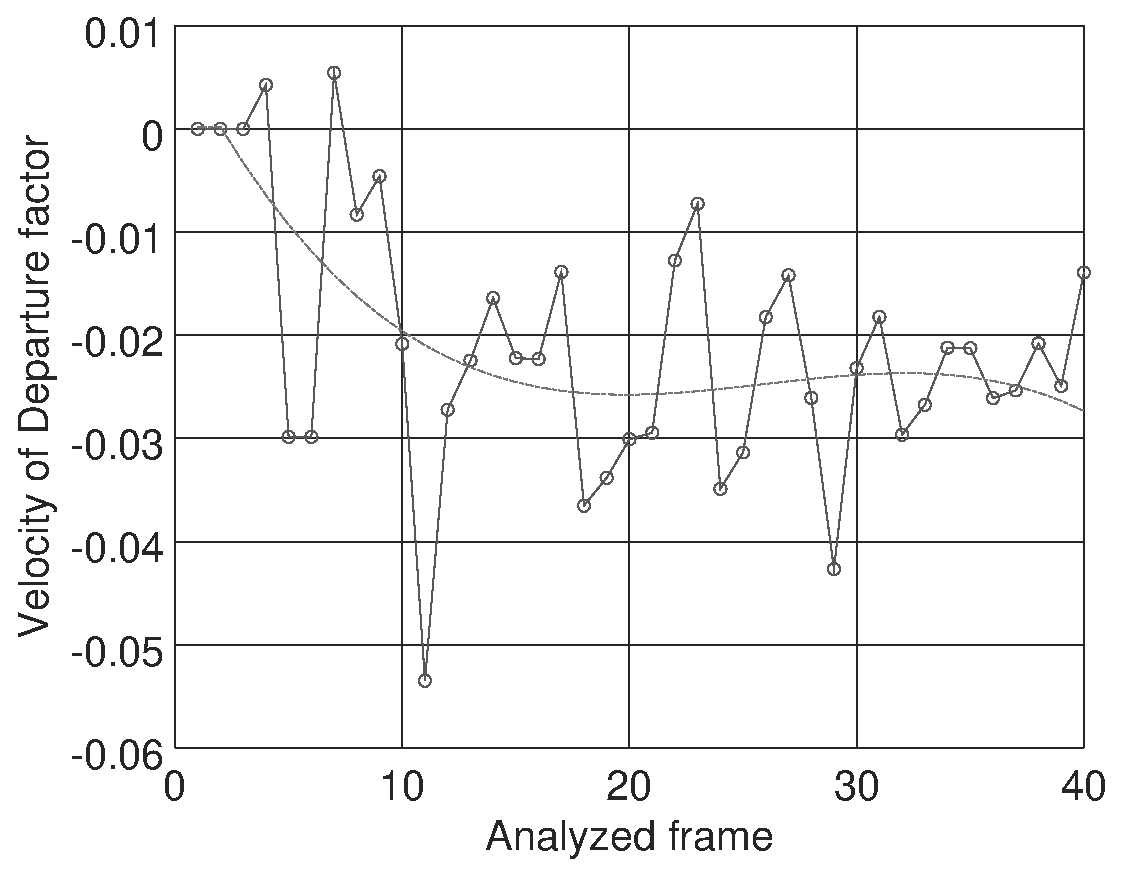
\includegraphics[width=\columnwidth]{images/graphvelocity.eps}
\caption{Velocidade do fator de aproximação para cada imagem no teste 2.}
\label{fig:res_grapha_bv}
\end{figure}